\chapter{Analysis of performance}

The time of the simulation will be used to characterize the performance when 
several parameters are changed. The time is measured using the wall clock, and 
refers to the \textit{time per iteration}. Sometimes the different stages of the 
simulator will be measured as well, to give more insight in the distribution of 
the time. Notice that each process may start or end a iteration at different 
times, by in the long run all processes must be synchronized. The measurements 
will take place only in the first process (with rank zero).

At each iteration various factors may affect the iteration time and introduce a 
random delay. We will model the simulation time as $t = \hat t + e_t$, where the 
true simulation time $\hat t$ is unknown but constant between iterations, and 
the error $e_t$ is a random variable with zero mean and unknown but finite 
variance $\sigma^2$.  Additionally, we will assume that the error $e_t$ is 
independent and identically distributed in each iteration of the same 
configuration and that follows a normal distribution.

We can consider the sequence of measured times $T = t_1,\ldots,t_n$ as 
independent random variables from a common distribution with an unknown mean 
$\hat t$ and finite standard deviation $\sigma$. The sample mean $\overline T$ 
can be approximated with a certain degree of confidence by a process of 
sampling. The standard error of the mean (SEM) will be used to get a confidence 
interval in which we can ensure the true mean is located. The standard error of 
the mean (SEM) is defined as
%
\begin{equation}
\epsilon = \frac{\sigma}{\sqrt{n}}
\end{equation}
%
As the standard deviation $\sigma$ is unknown, following the assumption that the 
error follows a normal distribution, we can use the student distribution to get 
the standard error using the standard deviation of the sample $s$
%
\begin{equation}
\epsilon = Z_\alpha\frac{s}{\sqrt{n}}
\end{equation}
%
With a significance level $\alpha=0.05$ we get from the t-student distribution 
the value $Z=1.96$, and we can obtain the confidence interval $\overline T \pm 
\epsilon$ where we can ensure the true mean is located with a probability of 
95\%. By setting the relative error $\delta = \epsilon / \overline T$ to be 
lower than 1\%, we obtain the limit error $\epsilon_0$ to be $\epsilon_0 = 0.01 
\overline T$.
%
Then, if we stop the simulation process when the standard error of the mean is 
below $\epsilon_0$
%
\begin{equation}
\epsilon = Z_\alpha\frac{s}{\sqrt{n}} < 0.01 \, \overline T
\end{equation}
%
We can ensure the following: (a) with probability 0.95, the true mean $\hat t$ 
is located in the interval $\overline T \pm \epsilon$, and (b) the relative 
error of the mean $\epsilon/\overline T$ is lower than 1\%.

The process of simulation will run for at least a minimum of 30 iterations. Then 
it will continue until the relative error is below 1\%.

\section{Performance model}

Consider the real time of the simulation $\hat t$ to be a function of a specific 
configuration $c$. There are a lot of parameters that may be changed and have 
some influence in the time per iteration, but we will focus only on the 
following ones.
%
\begin{enumerate}
\item $N_p$: Number of total particles.
\item $N_g$: Number of total grid points.
\item $N_c$: Number of plasma chunks.
\item $P$: Number of total MPI processes.
\item $C$: Number of total cores.
\end{enumerate}
%
A configuration is then completely specified as the tuple $c = (N_p, N_g, N_c, 
P, C)$.

Different parameters of the simulation may affect the time per iteration. At 
least we need to iterate over each particle $N_p$, so  we can ensure a minimum 
time in $O(N_p)$. We also know that the worst-case complexity of the FFT is in 
$O(N_g \log N_g)$ for $N_g$ total grid points.

\subsection{Number of particles}

The number of particles $N_p$ is one of the main parameters that affect the
running time of each iteration as it can be observed from the simulation process 
that at least a complexity in $O(N_p)$ is expected---we need to cycle through 
particle in each iteration. To get an accurate relation, an experiment is run 
sweeping from \num{2e6} to \num{4e7} particles, with 32 cores and only one 
process. The number of grid points is kept low at $1024^2$ grid points, in order 
to avoid interference from the solver. We see in the 
figure~\ref{fig:particles-32cpus} how the time scales linearly with the number 
of particles, and the residuals of the linear regression. With a determination 
coefficient of $R^2 = 0.99981$, we get a time per particle of 
\SI{51.42}{\micro\second} with 32 cores.


\begin{figure}[h]
	\centering
	\begin{tikzpicture}
	\begin{axis}[
		width=0.5\textwidth,
		xlabel=Particles $N_p$,
		ylabel=Time per iteration (s),
		no markers,
		%grid=major,
	]
	\addplot [only marks,scatter,error bars/y dir=both, error bars/y explicit] 
	table [
		x index = {0},
		y index = {3},
		y error index={4},
		col sep=space] {perf/particles/csv/time.csv};
	\addplot [red] table [col sep=space] {perf/particles/csv/regression.csv};
	\end{axis}
	\end{tikzpicture}
	\begin{tikzpicture}
	\begin{axis} [
		yticklabel pos=right,
		xlabel=Particles $N_g$,
		ylabel=Residuals (s),
		width=0.5\textwidth,
		%grid=major,
	]
	\addplot [
		only marks,
		error bars/y dir=both,
		error bars/y explicit,
	] table [
		x index = {0},
		y index = {2},
		y error index = {3},
		col sep=space] {perf/particles/csv/regression.csv};
	\draw[
		ultra thin,
		black!30!white
	] (axis cs:\pgfkeysvalueof{/pgfplots/xmin},0) --
			(axis cs:\pgfkeysvalueof{/pgfplots/xmax},0);
	\end{axis}
	\end{tikzpicture}
	\caption{The effect of the variables $N_p$ and $N_g$ to the time per 
	iteration. Using one process and 32 CPUs (MPI communications are not needed).}
	\label{fig:particles-32cpus}
\end{figure}

\begin{figure}[h]
	\centering
	\subfloat[Increasing number of grid points]{
		\begin{tikzpicture}
		\begin{axis} [
			no markers,
			grid=major,
			xlabel=Grid points $N_g$,
			ylabel=Time per iteration (s),
			width=0.5\textwidth]
		\addplot [only marks,error bars/y dir=both, error bars/y explicit] table [
			x index = {0},
			y index = {3},
			y error index={4},
			col sep=space] {perf/gridpoints/time.csv};
		\end{axis}
		\end{tikzpicture}
	}
	\caption{The effect of the variables $N_p$ and $N_g$ to the time per 
	iteration. Using one process and 32 CPUs (MPI communications are not needed).}
	\label{fig:particles-32cpus}
\end{figure}

\subsection{Constant number of CPUs}

The simulator is designed to scale with the number of particles when the number 
of CPUs or process are incremented, as each chunk can be computed in parallel.  
But when the number of grid points is incremented, the FFT solver must scale 
both in the number of CPUs and processes. The FFTW library offers two 
parallelization implementations for multithreading: Using OpenMP and POSIX 
threads (pthreads). OpenMP is not compatible with OmpSs-2 as we have one runtime 
already running so the pthread implementation was tested.
%
\begin{figure}[h]
	\centering
		\begin{tikzpicture}
		\begin{axis} [
			legend pos=north west,
			xmode=log,
			log basis x=2,
			xticklabels={0,1,2,4,8,16,32},
			grid=major,
			xlabel=Number of CPUs,
			ylabel=Time per iteration (s),
			width=10cm,
			height=6cm,
			]
		\addplot+ [only marks,error bars/y dir=both, error bars/y explicit] table [
			x index = {0},
			y index = {3},
			y error index={4},
			col sep=space] {perf/fftw-sequential/time.csv};
		\addlegendentry{Single thread}
		\addplot+ [only marks,error bars/y dir=both, error bars/y explicit] table [
			x index = {0},
			y index = {3},
			y error index={4},
			col sep=space] {perf/fftw-threads/time.csv};
		\addlegendentry{Multithread}
		\end{axis}
		\end{tikzpicture}
	\caption{The number of CPUs is increased with only one process: the solver 
	cannot scale and the time per iteration increases. Configuration used: $N_p = 
	\num{5e5}$, $N_g=8192\times8192$.}
	\label{fig:fftw-time}
\end{figure}
%
Unfortunately, the FFTW library doesn't show a good speedup, in fact worsens the 
time per iteration when adding more threads with the configurations tested. In 
the figure~\ref{fig:fftw-time} it can be shown how the time grows as the number 
of CPUs increases.
%
The FFTW documentation warns about this problem, claiming that it can only 
improve the time with large enough matrices:
%
\begin{displayquote}
A shared-memory machine is one in which all CPUs can directly access the same 
main memory, and such machines are now common due to the ubiquity of multi-core 
CPUs. FFTW’s multi-threading support allows you to utilize these additional CPUs 
transparently from a single program. However, this does not necessarily 
translate into performance gains---when multiple threads/CPUs are employed, 
there is an overhead required for synchronization that may outweigh the 
computational parallelism. Therefore, you can only benefit from threads if your 
problem is sufficiently large.
\end{displayquote}
%
However, larger matrices are not useful to get more precise results, as we 
rather prefer an increase in the number of particles than in grid points.


\begin{figure}[h]
	\centering
	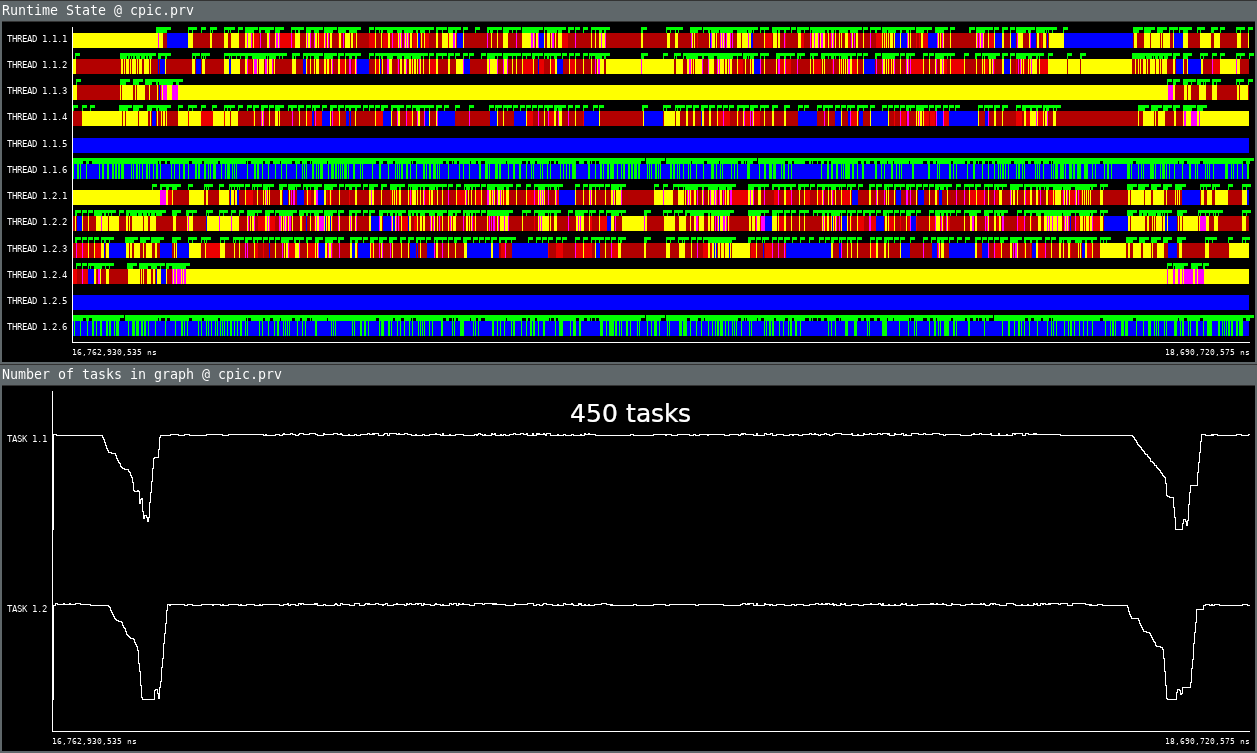
\includegraphics[width=0.95\linewidth]{fftw-ompss2.png}
	\caption{Tasks created inside the FFTW when using OmpSs-2: Up to 450 tasks are 
	created in rapid succession, with only 4 CPUs and 2 processes.}
	\label{fig:fftw-ompss2}
\end{figure}

In order to avoid a scalability problem, another approach was tested: Add 
support for OmpSs-2~in the FFTW to enable multithreading, following the same 
structure as OpenMP. The results obtained were similar as with the pthread case, 
but more insight was gained in how the task were created. It shown that the 
overhead added by the large amount of created and destructed quick tasks 
outweight any benefit that could be gained by multithreading.


We can mitigate the effect of the scaling by increasing the number of processes.  
In order to evaluate which ratio of processes and CPUs yields the best 
performance several configurations are tested. With a fixed number of maximum 
CPUs available set to 32, we increase the number of processes while we reduce 
the CPUs per process.


\begin{figure}[h]
	\centering
		\begin{tikzpicture}
		\begin{axis} [
			legend pos=outer north east,
			xmode=log,
			log basis x=2,
			xticklabels={0,1,2,4,8,16},
%			xticklabel style={
%			/pgf/number format/precision=3,
%			/pgf/number format/fixed},
			grid=major,
			xlabel=Number of CPUs per process,
			ylabel=Time per iteration (s),
			width=0.5\textwidth]
		\addplot [ybar stacked, fill=red!30!white] table [
			x index = {0},
			y index = {10},
			col sep=space] {perf/constant-cpus/time.csv};
		\addlegendentry{Solver}
		\addplot [ybar stacked, fill=blue!30!white] table [
			x index = {0},
			y index = {11},
			col sep=space] {perf/constant-cpus/time.csv};
		\addlegendentry{Particles}
		\addplot [only marks,error bars/y dir=both, error bars/y explicit] table [
			x index = {0},
			y index = {5},
			y error index={6},
			col sep=space] {perf/constant-cpus/time.csv};
		\addlegendentry{Total}
		\end{axis}
		\end{tikzpicture}
	\caption{The number of CPUs per process is incremented while reducing the 
	number of processes (the total number of CPUs is set to 32 and is kept 
	constant).  The time per iteration is measured, which leads to a 
	characteristic U shape.}
\end{figure}

%\begin{figure}[h]{{{
%	\centering
%		\begin{tikzpicture}
%		\begin{axis} [
%			baseline,
%			xmode=log,
%			log basis x=2,
%			xticklabels={0,1,2,4,8,16},
%%			xticklabel style={
%%			/pgf/number format/precision=3,
%%			/pgf/number format/fixed},
%			grid=major,
%			xlabel=Number of CPUs per process,
%			ylabel=Time per iteration (s),
%			ymax=6,
%			width=0.5\textwidth,
%			height=10cm,
%			]
%		\foreach \Nc in {32,64,128,256,512} {
%			\edef\temp{\noexpand\addlegendentry{$N_c = \Nc$}}
%			\addplot+ table [
%				x = P,
%				y = mean,
%				y error = {rel-err},
%				col sep=tab] {csv/mpi-scaling/Nc\Nc};
%			%\temp
%		}
%		\end{axis}
%		\end{tikzpicture}
%		\hspace{0.15cm}
%		\begin{tikzpicture}
%		\begin{axis} [
%			baseline,
%			xmode=log,
%			log basis x=2,
%			xticklabels={0,1,2,4,8,16},
%%			xticklabel style={
%%			/pgf/number format/precision=3,
%%			/pgf/number format/fixed},
%			grid=major,
%			xlabel=Number of CPUs per process,
%			ylabel=Time per iteration (s),
%			height=10cm,
%			width=0.5\textwidth]
%		\foreach \Nc in {32,64,128,256,512} {
%			\edef\temp{\noexpand\addlegendentry{$N_c = \Nc$}}
%			\addplot+ table [
%				x = P,
%				y = mean,
%				y error = {rel-err},
%				col sep=tab] {csv/tampi-scaling/Nc\Nc};
%			\temp
%		}
%		\end{axis}
%		\end{tikzpicture}
%	\caption{The number of CPUs per process is incremented while reducing the 
%	number of processes (the total number of CPUs is set to 32 and is kept 
%	constant).  The time per iteration is measured, which leads to a 
%	characteristic U shape.}
%\end{figure}}}}

\begin{figure}
\centering
\begin{tikzpicture}
	\begin{groupplot}[
		group style={
			columns=2,
%			rows=2,
			horizontal sep=0.5cm,
			ylabels at=edge left,
			yticklabels at=edge left,
		},
		xmode=log,
		log basis x=2,
%		xticklabels={0,1,2,4,8,16},
		grid=major,
		xmin=0,
		ymin=0,
		xlabel=Number of processes,
		ylabel=Time per iteration (s),
		height=10cm,
		width=7cm,
		/tikz/font=\small]
	\nextgroupplot[ymax=6,title={MPI}]
	\foreach \Nc in {32,64,128,256,512} {
		\edef\temp{\noexpand\addlegendentry{$N_c = \Nc$}}
		\addplot+ table [
			x = P,
			y = mean,
			y error = {rel-err},
			col sep=tab] {perf/mpi-scaling/csv/Nc\Nc};
		%\temp
	}
% Using inout is slightly slower than commutative
%	\nextgroupplot[ymax=6,title={MPI with inout}]
%	\foreach \Nc in {32,64,128,256,512} {
%		\edef\temp{\noexpand\addlegendentry{$N_c = \Nc$}}
%		\addplot+ table [
%			x = P,
%			y = mean,
%			y error = {rel-err},
%			col sep=tab] {csv/mpi-inout-scaling/Nc\Nc};
%		%\temp
%	}
	\nextgroupplot[ymax=6,title={TAMPI}]
	\foreach \Nc in {32,64,128,256,512} {
		\edef\temp{\noexpand\addlegendentry{$N_c = \Nc$}}
		\addplot+ table [
			x = P,
			y = mean,
			y error = {rel-err},
			col sep=tab] {perf/tampi-scaling/csv/Nc\Nc};
		\temp
	}
	\end{groupplot}
\end{tikzpicture}
\end{figure}


\begin{figure}
\centering
\begin{tikzpicture}
	\begin{axis}[
		xmode=log,
		log basis x=2,
		xticklabels={0,1,2,4,8,16,32},
		grid=major,
		xmin=0,
		ymin=0,
		xlabel=Number of processes,
		ylabel=Time per iteration (s),
		height=10cm,
		width=0.5\textwidth,
		/tikz/font=\small]
		\addplot+ table [
			x = P,
			y = speedup,
			col sep=tab] {perf/strong-scaling/csv/time.csv};
	\end{axis}
\end{tikzpicture}
\begin{tikzpicture}
	\begin{axis}[
		xmode=log,
		log basis x=2,
		xticklabels={0,1,2,4,8,16,32},
		grid=major,
		xmin=0,
		ymin=0,
		xlabel=Number of processes,
		ylabel=Time per iteration (s),
		height=10cm,
		width=0.5\textwidth,
		/tikz/font=\small]
		\addplot+ table [
			x = P,
			y = efficiency,
			col sep=tab] {perf/strong-scaling/csv/time.csv};
	\end{axis}
\end{tikzpicture}
\end{figure}

